%%\subsection{VPNs}
\subsubsection{IPSec}
\label{section:IPSECgeneral}

% ciphersuites current 2013-12-09
\begin{description}

\item[Settings:] \mbox{}

\paragraph*{Assumptions}\mbox{}\\

We assume the use of IKE (v1 or v2) and ESP for this document.

\paragraph*{Authentication}\mbox{}\\

IPSEC authentication should optimally be performed via RSA signatures,
with a key size of 2048 bits or more. Configuring only the trusted CA
that issued the peer certificate provides for additional protection
against fake certificates.

If you need to use Pre-Shared Key authentication:

\begin{enumerate}
\item Choose a \textbf{random}, \textbf{long enough} PSK (see below)
\item Use a \textbf{separate} PSK for any IPSEC connection
\item Change the PSKs regularily
\end{enumerate}

The size of the PSK should not be shorter than the output size of
the hash algorithm used in IKE \footnote{It is used in a HMAC, see
RFC2104\cite{rfc2104}.}.

For a key composed of upper- and lowercase letters, numbers, and two
additional symbols\footnote{64 possible values = 6 bits},
table~\ref{tab:IPSEC_psk_len} gives the minimum lengths in characters.

\begin{table}[h]
  \centering
  \small
  \begin{tabular}{lc}
    \toprule
    IKE Hash & PSK length \\
    \midrule
    SHA256 & 43 \\
    SHA384 & 64 \\
    SHA512 & 86 \\
    \bottomrule
  \end{tabular}
  \caption{PSK lengths}
  \label{tab:IPSEC_psk_len}
\end{table}

\paragraph*{Cryptographic Suites}\mbox{}\\

IPSEC Cryptographic Suites are pre-defined settings for all the items
of a configuration; they try to provide a balanced security level and
make setting up VPNs easier.
\footnote{RFC6379\cite{rfc6379}, RFC4308\cite{rfc4308}}

When using any of those suites, make sure to enable ``Perfect Forward
Secrecy`` for Phase 2, as this is not specified in the suites. The
equivalents to the recommended ciphers suites in section
\ref{section:recommendedciphers} are shown in
table~\ref{tab:IPSEC_suites}.

\begin{table}[h]
  \centering
  \small
  \begin{tabular}{p{2.5cm}p{2.5cm}l}
    \toprule
    Configuration A & Configuration B & Notes\\
    \midrule
    \verb|Suite-B-GCM-256| &
    \verb|Suite-B-GCM-128| \newline
    \verb|VPN-B| 
    & All Suite-B variants use NIST elliptic curves\\
    \bottomrule
  \end{tabular}
  \caption{IPSEC Cryptographic Suites}
  \label{tab:IPSEC_suites}
\end{table}

\paragraph*{IKE or Phase 1}\mbox{}\\

Alternatively to the pre-defined cipher suites, you can define your
own, as described in this and the next section.

IKE or Phase 1 is the mutual authentication and key exchange phase;
table~\ref{tab:IPSEC_ph1_params} shows the parameters.

Use only ``main mode``, as ``aggressive mode`` has known security
vulnerabilities \footnote{\url{http://ikecrack.sourceforge.net/}}.

\begin{table}[h]
  \centering
  \small
  \begin{tabular}{lll}
    \toprule
    & Configuration A & Configuration B \\
    \midrule
    Mode & Main Mode & Main Mode \\
    Encryption & AES-256 & AES, CAMELLIA (-256 or -128) \\
    Hash & SHA2-* & SHA2-*, SHA1 \\
    DH Group & Group 14--18, 19--21 & Group 14--21 \\
%    Lifetime & \todo{need recommendations; 1 day seems to be common
%      practice} & \\
    \bottomrule
  \end{tabular}
  \caption{IPSEC Phase 1 parameters}
  \label{tab:IPSEC_ph1_params}
\end{table}

\paragraph*{ESP or Phase 2}\mbox{}\\

ESP or Phase 2 is where the actual data are protected; recommended
parameters are shown in table \ref{tab:IPSEC_ph2_params}.

\begin{table}[h]
  \centering
  \small
  \begin{tabular}{lll}
    \toprule
    & Configuration A & Configuration B \\
    \midrule
    Perfect Forward Secrecy & yes & yes \\
    Encryption & 
    \parbox[t]{5cm}{\raggedright
    \mbox{AES-GCM-16}, \mbox{AES-CTR}, \mbox{AES-CCM-16}, \mbox{AES-256}}
    &
    \parbox[t]{5cm}{\raggedright
    \mbox{AES-GCM-16}, \mbox{AES-CTR}, \mbox{AES-CCM-16}, \mbox{AES-256}, \mbox{CAMELLIA-256}, \mbox{AES-128}, \mbox{CAMELLIA-128}} \\
    Hash & SHA2-* (or none for AES-GCM) & SHA2-*, SHA1 (or none for AES-GCM) \\
    DH Group & Same as Phase 1 & Same as Phase 1 \\
%    Lifetime & \todo{need recommendations; 1-8 hours is common} & \\
    \bottomrule
  \end{tabular}
  \caption{IPSEC Phase 2 parameters}
  \label{tab:IPSEC_ph2_params}
\end{table}

\item[References:] \mbox{}

``A Cryptographic Evaluation of IPsec'', Niels Ferguson and Bruce
  Schneier: \url{https://www.schneier.com/paper-ipsec.pdf}

\end{description}

\subsubsection{Check Point FireWall-1}
   
\begin{description}
\item[Tested with Version:] \mbox{}

\begin{itemize}
\item R77 (should work with any currently supported version)
\end{itemize}

\item[Settings:] \mbox{}

Please see section \ref{section:IPSECgeneral} for guidance on
parameter choice. In this section, we will configure a strong setup
according to ``Configuration A''.

This is based on the concept of a ``VPN Community'', which has all the
settings for the gateways that are included in that community.
Communities can be found in the ``IPSEC VPN'' tab of SmartDashboard.

\begin{figure}[p]
  \centering
  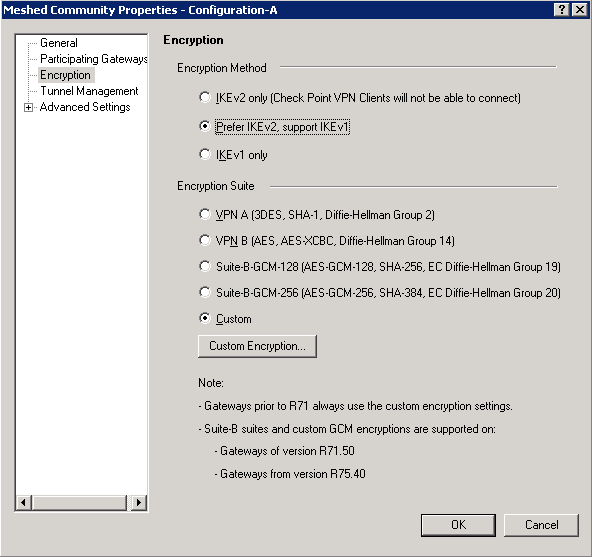
\includegraphics[width=0.592\textwidth]{checkpoint_1.png}
  \caption{VPN Community encryption properties}
  \label{fig:checkpoint_1}
\end{figure}

Either chose one of the encryption suites in the properties dialog
(figure \ref{fig:checkpoint_1}), or proceed to
``Custom Encryption...'', where you can set encryption and hash for
Phase 1 and 2 (figure \ref{fig:checkpoint_2}).

\begin{figure}[p]
  \centering
  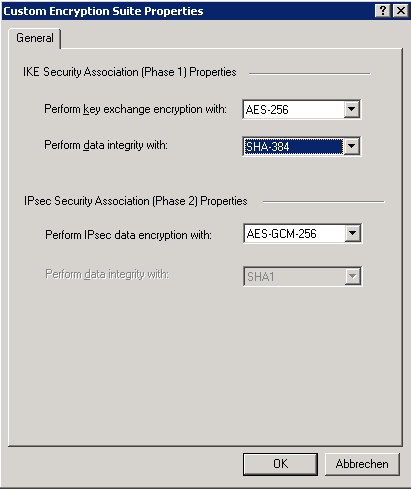
\includegraphics[width=0.411\textwidth]{checkpoint_2.png}
  \caption{Custom Encryption Suite Properties}
  \label{fig:checkpoint_2}
\end{figure}

The Diffie-Hellman groups and Perfect Forward Secrecy Settings can be
found under ``Advanced Settings'' / ``Advanced VPN Properties''
(figure \ref{fig:checkpoint_3}).

\begin{figure}[p]
  \centering
  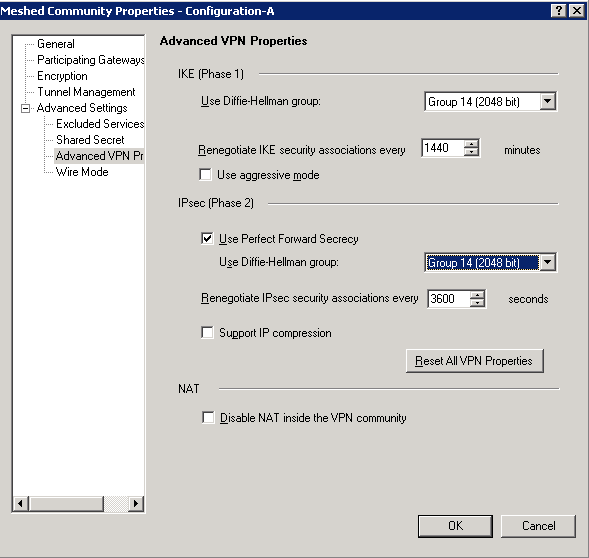
\includegraphics[width=0.589\textwidth]{checkpoint_3.png}
  \caption{Advanced VPN Properties}
  \label{fig:checkpoint_3}
\end{figure}

\item[Additional settings:] \mbox{}

For remote Dynamic IP Gateways, the settings are not taken from the
community, but set in the ``Global Properties'' dialog under ``Remote
Access'' / ``VPN Authentication and Encryption''. Via the ``Edit...''
button, you can configure sets of algorithms that all gateways support
(figure \ref{fig:checkpoint_4}).

\begin{figure}[p]
  \centering
  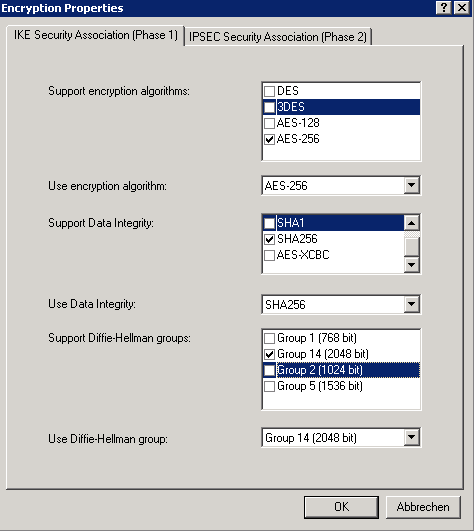
\includegraphics[width=0.474\textwidth]{checkpoint_4.png}
  \caption{Remote Access Encryption Properties}
  \label{fig:checkpoint_4}
\end{figure}

Please note that these settings restrict the available algorithms for
\textbf{all} gateways, and also influence the VPN client connections.

%\item[Justification for special settings (if needed):]

%\item[Limitations:]

\item[References:]\mbox{}

\begin{itemize}

\item Check Point
  \href{https://sc1.checkpoint.com/documents/R77/CP_R77_VPN_AdminGuide/html_frameset.htm}{VPN
    R77 Administration Guide} (may require a
  UserCenter account to access)

\end{itemize}

% \item[How to test:]

\end{description}


%% cipherstrings current 2013-12-09
\subsubsection{OpenVPN}

\begin{description}

\item[Tested with Version:] \mbox{}\\

\begin{itemize}
\item OpenVPN 2.3.2 from Debian ``wheezy-backports'' linked against openssl (libssl.so.1.0.0) 
\item OpenVPN 2.2.1 from Debian 7.0 linked against openssl
    (libssl.so.1.0.0) 
\item OpenVPN 2.3.2 for Windows
\end{itemize}

\item[Settings:] \mbox{}

\paragraph{General}\mbox{}

We describe a configuration with certificate-based authentication; see
below for details on the \verb|easyrsa| tool to help you with that.

OpenVPN uses TLS only for authentication and key exchange. The
bulk traffic is then encrypted and authenticated with the OpenVPN
protocol using those keys.

Note that while the \verb|tls-cipher| option takes a list of ciphers
that is then negotiated as usual with TLS, the \verb|cipher|
and \verb|auth| options both take a single argument that must match on
client and server.

\paragraph{Server Configuration}\mbox{}

% this is only a DoS-protection, out of scope:
% # TLS Authentication
% tls-auth ta.key

% previous:
% tls-cipher
% ECDHE-RSA-AES256-GCM-SHA384:ECDHE-RSA-AES256-SHA384:DHE-RSA-AES256-GCM-SHA384:DHE-RSA-AES256-SHA256:DHE-RSA-CAMELLIA256-SHA:ECDHE-RSA-AES256-SHA:DHE-RSA-AES256-SHA:AES256-SHA
% the cipherlist here is config B without the ECDHE strings, because
% it must fit in 256 bytes...
\begin{lstlisting}[breaklines]
tls-cipher DHE-RSA-AES256-GCM-SHA384:DHE-RSA-AES256-SHA256:DHE-RSA-AES128-GCM-SHA256:DHE-RSA-AES128-SHA256:DHE-RSA-CAMELLIA256-SHA:DHE-RSA-AES256-SHA:DHE-RSA-CAMELLIA128-SHA:DHE-RSA-AES128-SHA:CAMELLIA256-SHA:AES256-SHA:CAMELLIA128-SHA:AES128-SHA
cipher AES-256-CBC
auth SHA384
# generate with 'openssl dhparam -out dh2048.pem 2048':
dh dh2048.pem
\end{lstlisting}

\paragraph{Client Configuration}\mbox{}

Client and server have to use compatible configurations, otherwise they can't communicate.
The \verb|cipher| and \verb|auth| directives have to be identical.

\begin{lstlisting}[breaklines]
tls-cipher DHE-RSA-AES256-GCM-SHA384:DHE-RSA-AES256-SHA256:DHE-RSA-AES128-GCM-SHA256:DHE-RSA-AES128-SHA256:DHE-RSA-CAMELLIA256-SHA:DHE-RSA-AES256-SHA:DHE-RSA-CAMELLIA128-SHA:DHE-RSA-AES128-SHA:CAMELLIA256-SHA:AES256-SHA:CAMELLIA128-SHA:AES128-SHA
cipher AES-256-CBC
auth SHA384

# http://openvpn.net/index.php/open-source/documentation/howto.html#mitm
remote-cert-tls server

tls-remote server.example.com
\end{lstlisting}

\item[Justification for special settings (if needed):] \mbox{}\\

OpenVPN 2.3.1 changed the values that the \verb|tls-cipher| option
expects from OpenSSL to IANA cipher names. That means from that
version on you will get ``Deprecated TLS cipher name'' warnings for
the configurations above. You cannot use the selection strings from
section \ref{section:recommendedciphers} directly from 2.3.1 on, which
is why we give an explicit cipher list here.

In addition, there is a 256 character limit on configuration file line
lengths; that limits the size of cipher suites, so we dropped all
ECDHE suites.

The configuration shown above is compatible with all tested versions.

\item[References:] \mbox{}\\

\url{http://openvpn.net/index.php/open-source/documentation/security-overview.html}

%\item[How to test:]


\item[Additional settings:] \mbox{}

\paragraph{Key renegotiation interval}\mbox{}

The default for renegotiation of encryption keys is one hour
(\verb|reneg-sec 3600|). If you
transfer huge amounts of data over your tunnel, you might consider
configuring a shorter interval, or switch to a byte- or packet-based
interval (\verb|reneg-bytes| or \verb|reneg-pkts|).

\paragraph{Fixing ``easy-rsa''}\mbox{}

When installing an OpenVPN server instance, you are probably using
{\it easy-rsa} to generate keys and certificates.
The file \verb|vars| in the easyrsa installation directory has a
number of settings that should be changed to secure values:

\begin{lstlisting}[breaklines]
export KEY_SIZE=4096
export KEY_EXPIRE=365
export CA_EXPIRE=1826
\end{lstlisting}

This will enhance the security of the key generation by using RSA keys
with a length of 2048 bits, and set a lifetime of one year for the
server/client certificates and five years for the CA certificate.

In addition, edit the \verb|pkitool| script and replace all occurences
of \verb|sha1| with \verb|sha256|, to sign the certificates with
SHA256.

\item[Limitations:] \mbox{}

Note that the ciphersuites shown by \verb|openvpn --show-tls| are {\it
known}, but not necessarily {\it
supported} \footnote{\url{https://community.openvpn.net/openvpn/ticket/304}}.

Which cipher suite is actually used can be seen in the logs:

\verb|Control Channel: TLSv1, cipher TLSv1/SSLv3 DHE-RSA-CAMELLIA256-SHA, 2048 bit RSA|

\end{description}


\subsubsection{PPTP}

PPTP is considered insecure, Microsoft recommends to ``use a more secure VPN
tunnel''\footnote{\url{http://technet.microsoft.com/en-us/security/advisory/2743314}}.

There is a cloud service that cracks the underlying MS-CHAPv2
authentication protocol for the price of USD~200\footnote{\url{https://www.cloudcracker.com/blog/2012/07/29/cracking-ms-chap-v2/}},
and given the resulting MD4 hash, all PPTP traffic for a user can
be decrypted.

\subsubsection{Cisco ASA}
The following settings reflect our recommendations as best as possible on the Cisco ASA platform. These are - of course - just settings regarding SSL/TLS (i.e. Cisco AnyConnect) and IPSec. For further security settings regarding this platform the appropriate Cisco guides should be followed.
\begin{description}
\item[Tested with Version:] 
9.1(3) - X-series model
\item[Settings:] \mbox{}
\begin{lstlisting}[breaklines]
crypto ipsec ikev2 ipsec-proposal AES-Fallback
 protocol esp encryption aes-256 aes-192 aes
 protocol esp integrity sha-512 sha-384 sha-256
crypto ipsec ikev2 ipsec-proposal AES-GCM-Fallback
 protocol esp encryption aes-gcm-256 aes-gcm-192 aes-gcm
 protocol esp integrity sha-512 sha-384 sha-256
crypto ipsec ikev2 ipsec-proposal AES128-GCM
 protocol esp encryption aes-gcm
 protocol esp integrity sha-512
crypto ipsec ikev2 ipsec-proposal AES192-GCM
 protocol esp encryption aes-gcm-192
 protocol esp integrity sha-512
crypto ipsec ikev2 ipsec-proposal AES256-GCM
 protocol esp encryption aes-gcm-256
 protocol esp integrity sha-512
crypto ipsec ikev2 ipsec-proposal AES
 protocol esp encryption aes
 protocol esp integrity sha-1 md5
crypto ipsec ikev2 ipsec-proposal AES192
 protocol esp encryption aes-192
 protocol esp integrity sha-1 md5
crypto ipsec ikev2 ipsec-proposal AES256
 protocol esp encryption aes-256
 protocol esp integrity sha-1 md5
crypto ipsec ikev2 sa-strength-enforcement
crypto ipsec security-association pmtu-aging infinite
crypto dynamic-map SYSTEM_DEFAULT_CRYPTO_MAP 65535 set pfs group14
crypto dynamic-map SYSTEM_DEFAULT_CRYPTO_MAP 65535 set ikev2 ipsec-proposal AES256-GCM AES192-GCM AES128-GCM AES-GCM-Fallback AES-Fallback
crypto map Outside-DMZ_map 65535 ipsec-isakmp dynamic SYSTEM_DEFAULT_CRYPTO_MAP
crypto map Outside-DMZ_map interface Outside-DMZ

crypto ikev2 policy 1
 encryption aes-gcm-256
 integrity null
 group 24 14
 prf sha512 sha384 sha256 sha
 lifetime seconds 86400
crypto ikev2 policy 2
 encryption aes-gcm-256 aes-gcm-192 aes-gcm
 integrity null
 group 24 14
 prf sha512 sha384 sha256 sha
 lifetime seconds 86400
crypto ikev2 policy 3
 encryption aes-256 aes-192 aes
 integrity sha512 sha384 sha256
 group 24 14
 prf sha512 sha384 sha256 sha
 lifetime seconds 86400
crypto ikev2 policy 4
 encryption aes-256 aes-192 aes
 integrity sha512 sha384 sha256 sha
 group 24 14
 prf sha512 sha384 sha256 sha
 lifetime seconds 86400
crypto ikev2 enable Outside-DMZ client-services port 443
crypto ikev2 remote-access trustpoint ASDM_TrustPoint0

ssl server-version tlsv1-only
ssl client-version tlsv1-only
ssl encryption dhe-aes256-sha1 dhe-aes128-sha1 aes256-sha1 aes128-sha1
ssl trust-point ASDM_TrustPoint0 Outside-DMZ
\end{lstlisting}

\item[Justification for special settings (if needed):] \mbox{}
New IPsec policies have been defined which do not make use of ciphers that may be cause for concern. Policies have a "Fallback" option to support legacy devices.

3DES has been completely disabled as such Windows XP AnyConnect Clients will no longer be able to connect.

The Cisco ASA platform does not currently support RSA Keys above 2048bits.

Legacy ASA models (e.g. 5505, 5510, 5520, 5540, 5550) do not offer the possibility to configure for SHA256/SHA384/SHA512 nor AES-GCM for IKEv2 proposals.

\item[References:] 
\url{http://www.cisco.com/en/US/docs/security/asa/roadmap/asaroadmap.html}\\
\url{http://www.cisco.com/web/about/security/intelligence/nextgen_crypto.html}

% add any further references or best practice documents here

%%\item[How to test:] 
% describe here or point the admin to tools (can be a simple footnote or \ref{} to  the tools section) which help the admin to test his settings.

\end{description}







%%\subsubsection{Juniper VPN}
%%\todo{write this subsubsection. AK: ask Hannes}


%%\begin{description}
%%\item[Tested with Version:] \todo{version?}

%%\item[Settings:] \mbox{}

%%\begin{lstlisting}[breaklines]
%%    %Here goes your setting string
%%\end{lstlisting}

%%\item[Additional settings:] \mbox{}

%Here you can add additional settings

%%\begin{lstlisting}[breaklines]
%%    %copy \& paste additional settings
%%\end{lstlisting}

%%\item[Justification for special settings (if needed):] \mbox{}

% in case you have the need for further justifications why you chose this and that setting or if the settings do not fit into the standard Variant A or Variant B schema, please document this here

%%\item[References:] \todo{add references}

% add any further references or best practice documents here

%%\item[How to test:]
% describe here or point the admin to tools (can be a simple footnote or \ref{} to  the tools section) which help the admin to test his settings.

%%\end{description}



\subsubsection{L2TP over IPSec}
\todo{write this subsubsection}


\begin{description}
\item[Tested with Version:] \todo{version?}

\item[Settings:] \mbox{}

\begin{lstlisting}[breaklines]
    %Here goes your setting string
\end{lstlisting}

\item[Additional settings:] \mbox{}

%Here you can add additional settings

\begin{lstlisting}[breaklines]
    %copy \& paste additional settings
\end{lstlisting}

\item[Justification for special settings (if needed):] \mbox{}

% in case you have the need for further justifications why you chose this and that setting or if the settings do not fit into the standard Variant A or Variant B schema, please document this here

\item[References:] \todo{add references}

% add any further references or best practice documents here

\item[How to test:]
% describe here or point the admin to tools (can be a simple footnote or \ref{} to  the tools section) which help the admin to test his settings.

\end{description}






\subsubsection{Racoon}
\todo{write this subsubsection}


\begin{description}
\item[Tested with Version:] \todo{version?}

\item[Settings:] \mbox{}

\begin{lstlisting}[breaklines]
    %Here goes your setting string
\end{lstlisting}

\item[Additional settings:] \mbox{}

%Here you can add additional settings

\begin{lstlisting}[breaklines]
    %copy \& paste additional settings
\end{lstlisting}

\item[Justification for special settings (if needed):] \mbox{}

% in case you have the need for further justifications why you chose this and that setting or if the settings do not fit into the standard Variant A or Variant B schema, please document this here

\item[References:] \todo{add references}

% add any further references or best practice documents here

\item[How to test:]
% describe here or point the admin to tools (can be a simple footnote or \ref{} to  the tools section) which help the admin to test his settings.

\end{description}
